\documentclass{article}

\usepackage{graphicx}
\usepackage{subcaption}
\usepackage[portrait]{geometry}
\geometry{total={8.5in,11in},left=0.25in, top=0.25in, right=0.25in}

\begin{document}

\begin{figure}[h!]
\centering
\begin{subfigure}[b]{0.35\linewidth}
  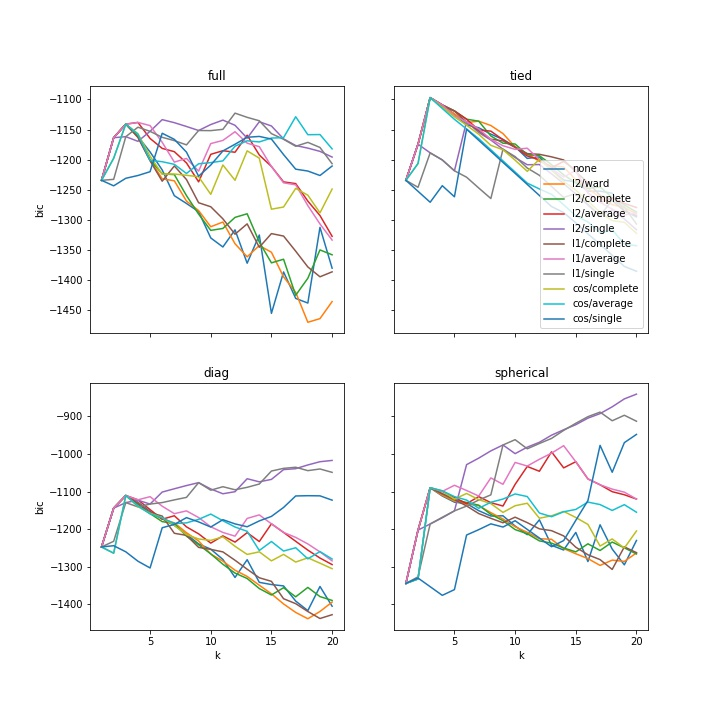
\includegraphics[width=\linewidth]{lowd_python_bicplot.jpg}
\caption{}
\end{subfigure}
\begin{subfigure}[b]{0.35\linewidth}
  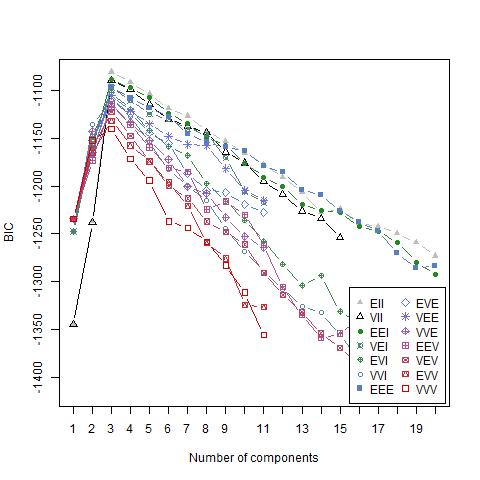
\includegraphics[width=\linewidth]{lowd_r_bicplot.jpg}
\caption{}
\end{subfigure} 
\begin{subfigure}[b]{0.35\linewidth}
  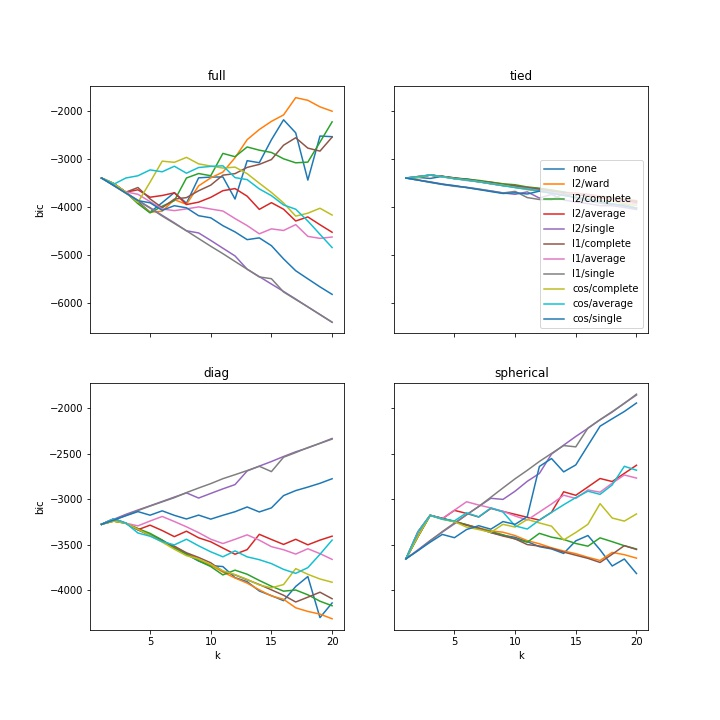
\includegraphics[width=\linewidth]{highd_python_bicplot.jpg}
\caption{}
\end{subfigure}
\begin{subfigure}[b]{0.35\linewidth}
  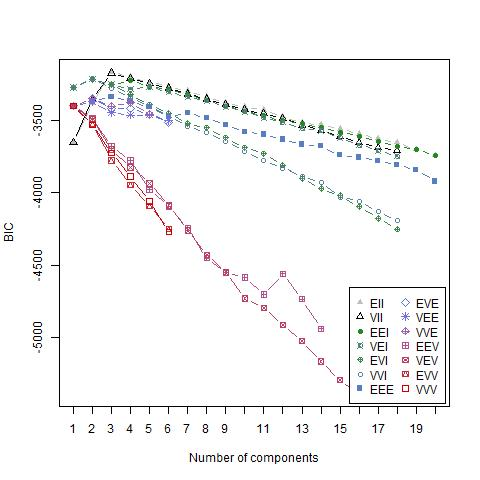
\includegraphics[width=\linewidth]{highd_r_bicplot.jpg}
\caption{}
\end{subfigure} 

\caption{BIC results on clustering a simple mixture of 3 Gaussians. The mixtures have identity covariance and have means at [0,0...],[5,0...],[0,5...]. a) pyclust results on 3d mixture b) mclust results on 3d mixture c) pyclust results on 10d mixture d) mclust results on 10d mixture}
\end{figure}



\end{document}